%% general_advice.tex
%% Author: Leighton Pritchard
%% Copyright: James Hutton Institute
%% Collected wisdom

% CAVEAT
\begin{frame}
  \frametitle{A word of caution}
  \begin{alertblock}{Rules are there to be broken}
  There are good reasons for breaking nearly every rule of presentation at one time or another.
  \end{alertblock}
\end{frame}

% USE THE FULL AXIS
\begin{frame}
  \frametitle{Use the full axis}
  \textcolor{hutton_blue}{but does difference from initial value matter more than absolute value?}
  \begin{center}
    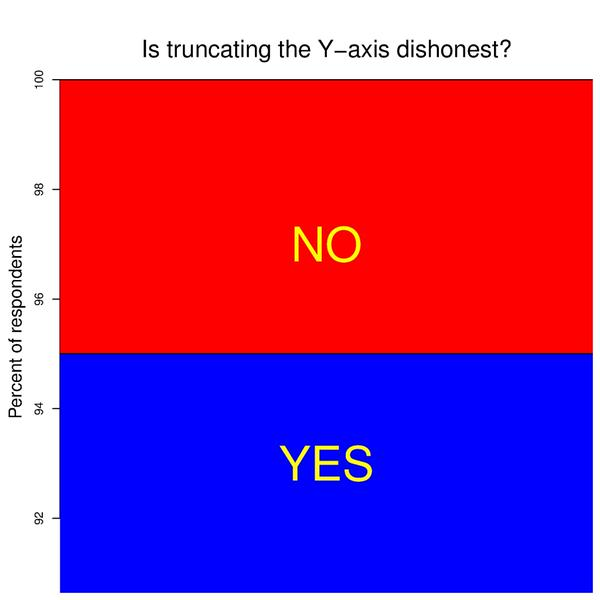
\includegraphics[width=0.35\textwidth,valign=c]{images/truncated_y}
    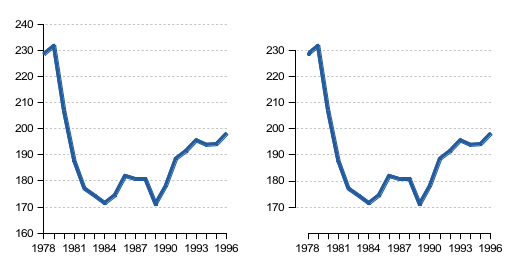
\includegraphics[width=0.65\textwidth,valign=c]{images/non-connected-axes}    
  \end{center}
\end{frame}

% SIMPLIFY
\begin{frame}
  \frametitle{Simplify to your message}
  \begin{center}
    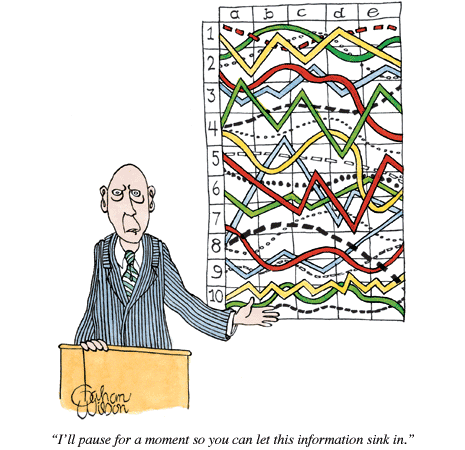
\includegraphics[width=0.45\textwidth,valign=t]{images/datavis_overcomplex}
    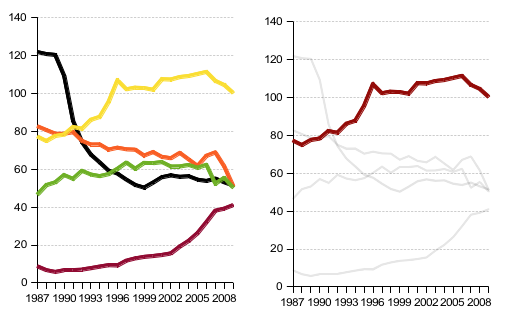
\includegraphics[width=0.55\textwidth,valign=t]{images/simplify}    
  \end{center}
\end{frame}